\only<presentation>{
\begin{frame}[label=uebersicht]{Kursus / Übersicht}
  \textbf{22.12.2017 : Internettechnologien II: von interaktiven Webseiten zu WebApps in der Cloud}
      \begin{itemize}
        \item Der Einsatz von JavaScript Frameworks anhand von Primos neuem UI
      \end{itemize}
\end{frame}
}
\section{Internettechnologien II: von interaktiven Webseiten zu WebApps in der Cloud}

\subsection{Das DOM}

\only<article>{
	Eine Webseite gliedert sich --- wie ,,normale‘‘ Textdokumente auch --- in verschiedene Abschnitte wie z.B. Überschriften, Absätze, es gibt Listen usw. Dazu kommen Bereiche im Layout wie z.B. Der Kopf, Randnotizen oder das Menü. All diese Elemente sind im DOM (document object model) beschrieben und darüber ansprechbar.
	Das DOM ist eine Spezifikation eines API, einer Programmierschnittstelle, mit der man html—Elemente ansprechen kann.
	Damit das funktioniert, müssen die Elemente im html—Dokument entsprechend ausgezeichnet sein.
  }

\begin{frame}[fragile]{Beispiele für Elemente im html--Dokument}
  \fontencoding{T1}\selectfont
  \begin{center}
    \begin{itemize}
      \item Überschriften : \lstinline[language=html] {<h1>Überschrift</h1>}
      \item Absätze : \lstinline[language=html] {<p>Absatz</p>}
      \item Tabellen : \lstinline[language=html] {<table><tr><td>Zelle</td></tr></table>} 
    \end{itemize}
  \end{center}
\end{frame}

\only<article>{
	Eine Unart war, die Dokumente mit Tabellen zu ,,gestalten‘‘ oder besser: zu verunstalten. Die Designer hatten erkannt, dass man mit Tabellen Text auf einer Webseite gut positionieren kann. Damit wird die Seite jedoch eher statisch, ist auf unterschiedlichen Monitorgrössen nicht mehr gleich gut lesbar, und unübersichtlich im Quelltext und damit schlecht zu pflegen. Diese Unart ist —- bis auf beim OPAC von Aleph -- inzwischen aus dem Netz verschwunden.
}

\begin{frame}{die Formatierung im alten OPAC}
  \begin{center}
    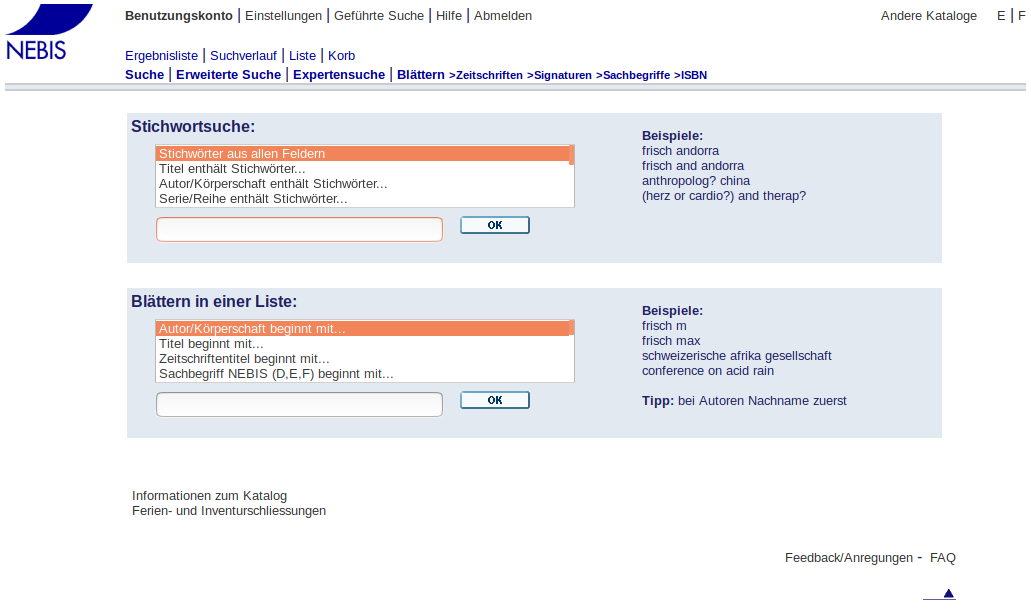
\includegraphics[width=1\textwidth]{pics/opac}
  \end{center}
\end{frame}

\begin{frame}[fragile]{die Formatierung im alten OPAC (Quelltext)}
  \fontencoding{T1}\selectfont
  \lstinputlisting[language=html]{html_und_js/20-opac-ausschnitt.html}
\end{frame}

\subsection{Das DOM für Gestaltungszwecke verwenden}
\only<article>{
  Dennoch bleibt natürlich der Wunsch, den hoffentlich wertvollen Inhalt auch ansprechend gestalten zu können. Dazu lassen sich die Elemente des DOMs mit Formatierungsinformationen versehen.
}

\begin{frame}[fragile]{unsere Webseite bis jetzt}
  \fontencoding{T1}\selectfont
  \begin{columns}[t,onlytextwidth]
    \begin{column}{0.7\textwidth}
      \lstinputlisting[language=html]{html_und_js/00-testseite-roh.html}
    \end{column}
    \begin{column}{0.3\textwidth}  %%<--- here
      \begin{center}
        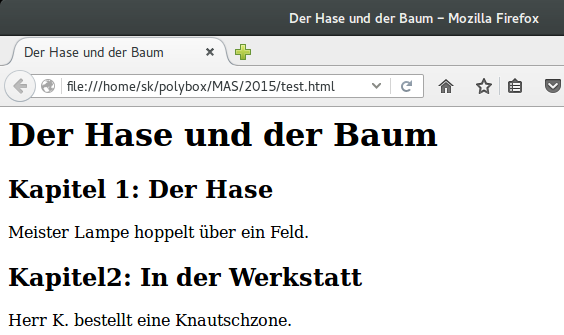
\includegraphics[width=1\textwidth]{pics/testseite-utf8}
      \end{center}
    \end{column}
  \end{columns}
\end{frame}

\only<article>{
  Eine Überschrift wird mit <h1> (bzw. h2,h3 usw.) ausgezeichnet. Dieser Auszeichnung kann man z.B. Formatierungsinformationen übergeben:
  }

\begin{frame}[fragile]{unsere Webseite bis jetzt}
  \fontencoding{T1}\selectfont
  Die Anweisung 

  \lstinline[language=html]{style="color: grey;"}
  
  lässt das entsprechende Element in grau erscheinen.
\end{frame}

\begin{frame}[fragile]{erste eigene Formatierung}
  \fontencoding{T1}\selectfont
  \begin{columns}[t,onlytextwidth]
    \begin{column}{0.7\textwidth}
      \lstinputlisting[language=html]{html_und_js/01-testseite-h1-styled.html}
    \end{column}
    \begin{column}{0.3\textwidth}  %%<--- here
      \begin{center}
        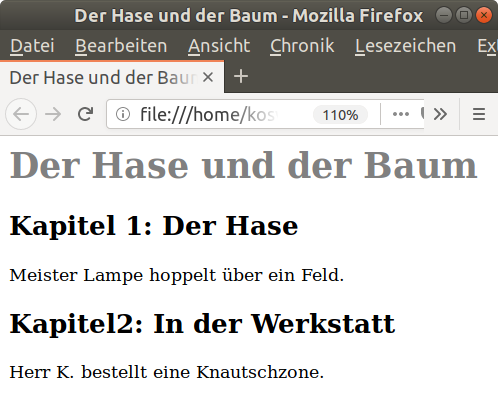
\includegraphics[width=1\textwidth]{pics/testseite-h1-styled}
      \end{center}
    \end{column}
  \end{columns}
\end{frame}

\only<article>{ 
Will man nun alle Überschriften in grau setzen, wird es etwas umständlich, wenn man die Informationen in jedes Element einzeln setzen müsste. Stattdessen kann man eine Formatierung, die für alle Elemente eines Typs gelten soll, zentral definieren:
}

\begin{frame}[fragile]{Formatierung im head}
  \fontencoding{T1}\selectfont
  \begin{columns}[t,onlytextwidth]
    \begin{column}{0.7\textwidth}
      \lstinputlisting[language=html]{html_und_js/02-testseite-formatiert.html}
    \end{column}
    \begin{column}{0.3\textwidth}  %%<--- here
      \begin{center}
        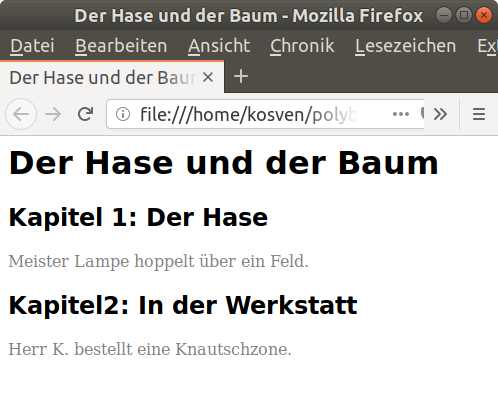
\includegraphics[width=1\textwidth]{pics/testseite-formatiert}
      \end{center}
    \end{column}
  \end{columns}
\end{frame}

\only<article>{
Da einzelne Elemente mehrfach vorkommen können, kann man sie zur eindeutigen Identifizierung mit einer ID versehen. 
Ausserdem kann man auch Klassen mit Formatierungsinformationen definieren, um so verschiedenen Elementen eine konsistente Formatierung zuweisen zu können.
Ein kompletter Webauftritt besteht nun selten nur aus einer Seite. Will man über mehrere Seiten ein konsistentes Layout erzielen, müsste man die Formatierungsinformationen im Header in jede Seite kopieren.

EXKURS ,,DRY‘‘

Das DRY--Prinzip verbietet es, die Formatierungsinformationen in jeder einzelnen Seite redundant vorzuhalten und jeweils einzeln pflegen zu müssen. Stattdessen lagert man sie in eine eigene Datei aus, die als stylesheet (css) im head der Seite verlinkt wird. 
}

\begin{frame}[fragile]{externes Stylesheet}
  \fontencoding{T1}\selectfont
  \begin{lstlisting}[language=html]
<head>
  <link rel="stylesheet" media="all" href="/assets/application-
    e77e74d6189491bd233e87f81af0db0315d8ed4a4e7b0070d13b6180200
    ce1a7.css">
</head>
  \end{lstlisting}
\end{frame}


\begin{frame}[fragile]{Auszug aus dem css von libraries.ch}
  \fontencoding{T1}\selectfont
  \begin{lstlisting}[language=html]
a, label, .btn {
  font-size: 1em
}

a {
  color: #20758c
}
...
body {
  font-size: 1em
  overflow-y: scroll
}
...
footer h3 {
  font-size: 1.2em
  margin-top: 0
  margin-bottom: 0
  height: 1.4em
}
  \end{lstlisting}
\end{frame}

\only<article>{
Da wir aber in unserem Beispiel nur eine einzelne Seite haben, lasse ich die Formatierungsinformationen ausnahmsweise im head.}

\subsection{Das DOM für JavaScript-Funktionen verwenden}
\label{sub:das_dom_für_javascript_funktionen}

\only<article>{
Man kann nun das DOM auch verwenden, um Elemente in der Seite vom Client, also vom Browser des Nutzers dynamisch anpassen zu lassen. Das probieren wir im Folgenden mal mit Hilfe der Entwicklertools im FireFox. Doch zunächst geben wir einer Tabellenzeile eine id.
}

\begin{frame}[fragile]{id vergeben}
  \fontencoding{T1}\selectfont
  \lstinputlisting[language=html]{html_und_js/10-javascript-id.html}
\end{frame}

\begin{frame}[fragile]{Element mit JavaScript ausblenden}
  \fontencoding{T1}\selectfont
  Der JavaScript--Befehl 

  \lstinline{document.getElementById("kapitel2").style.display = 'none';}

  blendet das Element mit der id ,,kapitel2'' aus.
\end{frame}

\only<article>{
  Um den Befehl eingeben zu können, müssen wir die Entwicklertools öffnen (Strg+Umschalt+I).
}

\begin{frame}{Die Entwicklertools}
  \begin{center}
    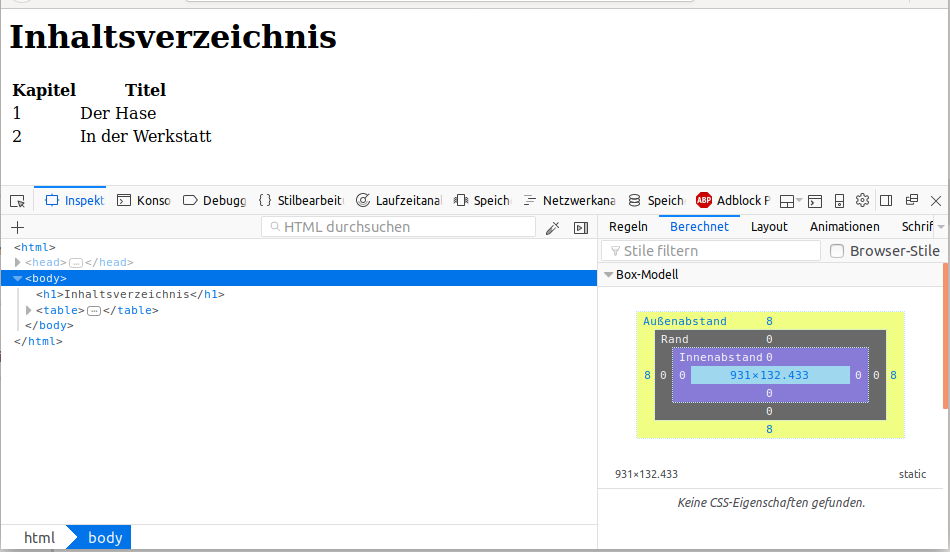
\includegraphics[width=1\textwidth]{pics/dev-tools}
  \end{center}
\end{frame}

\begin{frame}{Die Entwicklertools : Konsole}
  \begin{center}
    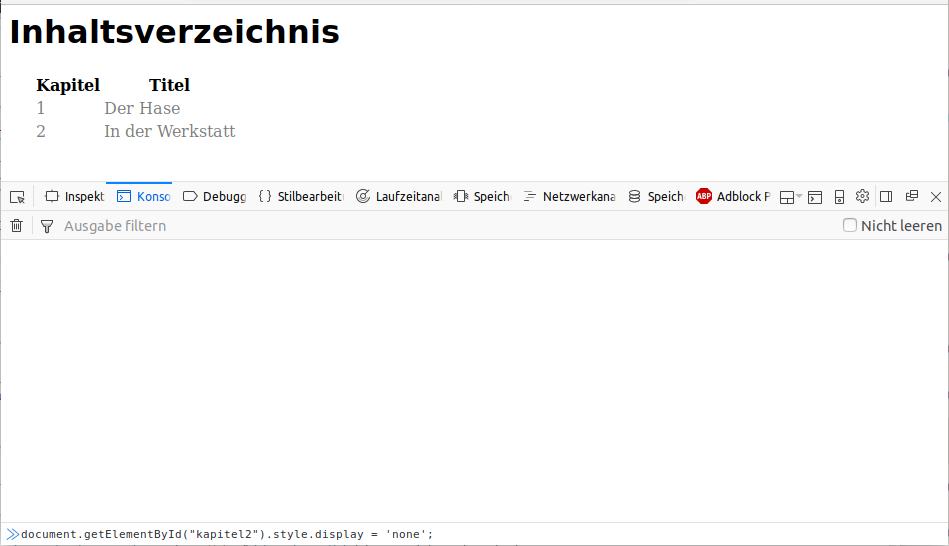
\includegraphics[width=1\textwidth]{pics/konsole}
  \end{center}
\end{frame}

\only<article>{
  Natürlich lässt man das nicht den Endbenutzer von Hand machen. Stattdessen wird ein entsprechendes JavaScript in die Seite eingebaut, das beispielsweise durch Klick auf ein Element ausgeführt wird. Im Beispiel verwenden wir einen einfachen Textlink:
}

\begin{frame}[fragile]{Element mit script ausblenden}
  \fontencoding{T1}\selectfont
  \lstinputlisting[language=html]{html_und_js/14-javascript.html}
  
  Und so sieht es \href{./html_und_js/15-javascript.html}{im Browser} aus:

\end{frame}

\begin{frame}[fragile]{Element mit script ein-- und ausblenden}
  \fontencoding{T1}\selectfont
  \lstinputlisting[language=html]{html_und_js/16-javascript.html}
  
  Und so sieht es \href{./html_und_js/17-javascript.html}{im Browser} aus:

\end{frame}
  
\only<article>{
  Übung / Spiel: Wie verhindern wir das Springen in der Tabellenkopfzeile?
    th { text-align: left; }

  Viele Probleme kommen immer wieder in ähnlicher Form vor. Man vereinfacht sich das, indem man Elemente so programmiert, dass sie wieder verwendbar sind. Ein guter Punkt, der sich mit der Entwicklung der objektorientierten Programmierung stark verbreitet hat. 

  Auf entsprechenden Plattformen werden Code--Schnipsel, Lösungen und komplette Programme ausgetauscht. (Github, Gitlab, Bitbucket...)
}

\subsection{JavaScript--Libraries und --FrameWorks}
\label{sub:libraries_und_frameworks}

\only<article>{
  Zurück zur Webseite: Auch hier kommen viele Elemente immer wieder vor und werden von vielen Entwicklern benötigt. Das Ein-- und Ausblenden von Elementen ist eine häufig gestellte Anforderung. Damit nun nicht jeder den Javascriptcode wieder schreiben (oder von Github kopieren) muss, gibt es Leute, die Lösungen zu ganzen Sammlungen zu einem Thema zusammen stellen, die sogenannten Bibliotheken bzw. ,,Libraries''. 

  Noch umfangreicher als Libraries sind FrameWorks, bei denen verschiedene Libraries, unterstützende Software und sogar Skriptsprachen zusammengepackt werden, um das Softwaredevelopment im entsprechenden Gebiet erheblich zu vereinfachen. 

  Die Grenzen sind fliessend und nicht eindeutig zu bestimmen. Man kann sicher sagen, dass FrameWorks wiederverwertbare Strukturen mit komplexen Anwendungen zur Programmierung und ein abstraktes Design bereit stellen, wohingegen eher Libraries Funktionssammlungen zu konkreten Aufgaben sind.
}

\begin{frame}{zwei verbreitete JavaScript Libraries}
  \begin{itemize}
    \item jquery / jquery UI
    \item bootstrap
  \end{itemize}
\end{frame}

\begin{frame}{zwei verbreitete JavaScript FrameWorks}
  \begin{itemize}
    \item AngularJS / Angular 2
    \item ReactJS
  \end{itemize}
\end{frame}

\only<article>{
  Libraries und FrameWorks bindet man in den head seiner Webseite ein. Der Nachteil ist, dass jeder Nutzer der Webseite sich einmal die komplette Library bzw. das komplette FrameWork (im Hintergrund) herunterladen muss, auch wenn man von tausenden Funktionen nur zwei benötigt.

  Es gibt verschiedene\ldots
  }

\begin{frame}{Möglichkeiten, JS einzubinden:}
  \begin{itemize}
    \item eine Version direkt auf dem eigenen Server zur Verfügung stellen
    \item eine bestimmte Version als Link direkt einbinden
    \item eine Minimalversion einbinden und benötigte Funktionen dynamisch nachladen (problematisch, wenn das Gerät nicht dauerhaft online ist)
  \end{itemize}
\end{frame}

\only<article>{
  Beginnen wir mit einem Beispiel, bei dem wir die Library ,,jquery'' direkt über einen Link zum Anbieter in der jeweils neuesten Version einbinden.
}

\begin{frame}[fragile]{die Einbindung von jquery}
  \fontencoding{T1}\selectfont
  \begin{lstlisting}[language=html]
<html>
  <head>
    <meta charset="utf-8" />
    <script src="https://code.jquery.com/jquery-latest.js"></script>
...
  \end{lstlisting}
\end{frame}

\only<article>{
  Der Link im Beispiel oben zeigt immer auf die aktuellste Version (,,jquery-latest.js''), was problematisch sein kann, falls es in einer neueren Version Änderungen gegeben hat, die nicht mit dem Code bzw. den Skripts in der Webseite kompatibel sind. Deswegen kann es sinnvoll sein, stattdessen auf eine konkrete Version zu verlinken bzw. diese direkt auf dem eigenen Webserver zur Verfügung zu stellen.

  jquery erlaubt nun ein viel einfacheres Ansteuern der DOM--Elemente, als pures JavaScript. Auch sind --- wie beschrieben --- oft benötigte Funktionen gleich integriert. So will man oftmals ein Element nicht nur einmal einblenden bzw. ausblenden, sondern wiederkehrend ein-- und ausblenden. jquery stellt hierfür die Funktion ,,toggle'' zur Verfügung.
}

\begin{frame}[fragile]{Das Ansteuern der Elemente ist viel einfacher}
  \fontencoding{T1}\selectfont

  Der Befehl

  \lstinline{$("#kapitel2").toggle();}

  blendet das Element mit der id ,,kapitel2'' ein und aus.

  \href{./html_und_js/18-javascript-jquery.html}{--> Test im Browser}
\end{frame}

\begin{frame}[fragile]{ein-- / ausblenden mit jquery}
  \fontencoding{T1}\selectfont
  \begin{lstlisting}[language=html]
...
  <tr>
    <td colspan="2"><a href="#" id="schalter">zeige</a></td>
  </tr>
  <tr id="kapitel2" style="display: none;">
    <td>2</td><td>In der Werkstatt</td>
  </tr>
</table>

<script type="text/javascript">
  $(document).ready(function(){
    $("#schalter").click(function(){
      $("#kapitel2").toggle();
    });
  });
</script>
...
  \end{lstlisting}
\end{frame}

\begin{frame}[fragile]{Userinterface mit jquery UI}
  \fontencoding{T1}\selectfont
  Mit der Bibliothek ,,jquery UI'' lassen sich schnell einheitliche Oberflächen bauen. 
  Hier ein \href{./html_und_js/19-javascript-jqueryui.html}{Button}:
  \begin{lstlisting}[language=html]
<head>
    <meta charset="utf-8" />
    <script src="https://code.jquery.com/jquery-latest.js"></script>
    <link rel="stylesheet" href="https://ajax.googleapis.com/ajax/libs/jqueryui/1.12.1/themes/smoothness/jquery-ui.css">
    <script src="https://ajax.googleapis.com/ajax/libs/jqueryui/1.12.1/jquery-ui.min.js"></script>
...
<body>
...
    <button>zeige Kapitel 2</button>}
  \end{lstlisting}
\end{frame}

\begin{frame}[fragile]{bootstrap statt Tabellenlayout}
  \fontencoding{T1}\selectfont
  \begin{lstlisting}
<div class="row">
  <div class="col-md-3">...</div>
  <div class="col-md-1">...</div>
  <div class="col-md-3">...</div>
  <div class="col-md-1">...</div>
  <div class="col-md-3">...</div>
  <div class="col-md-1">...</div>
</div>
  \end{lstlisting}
\end{frame}

\begin{frame}{auf einem normalen Monitor}
  \begin{center}
    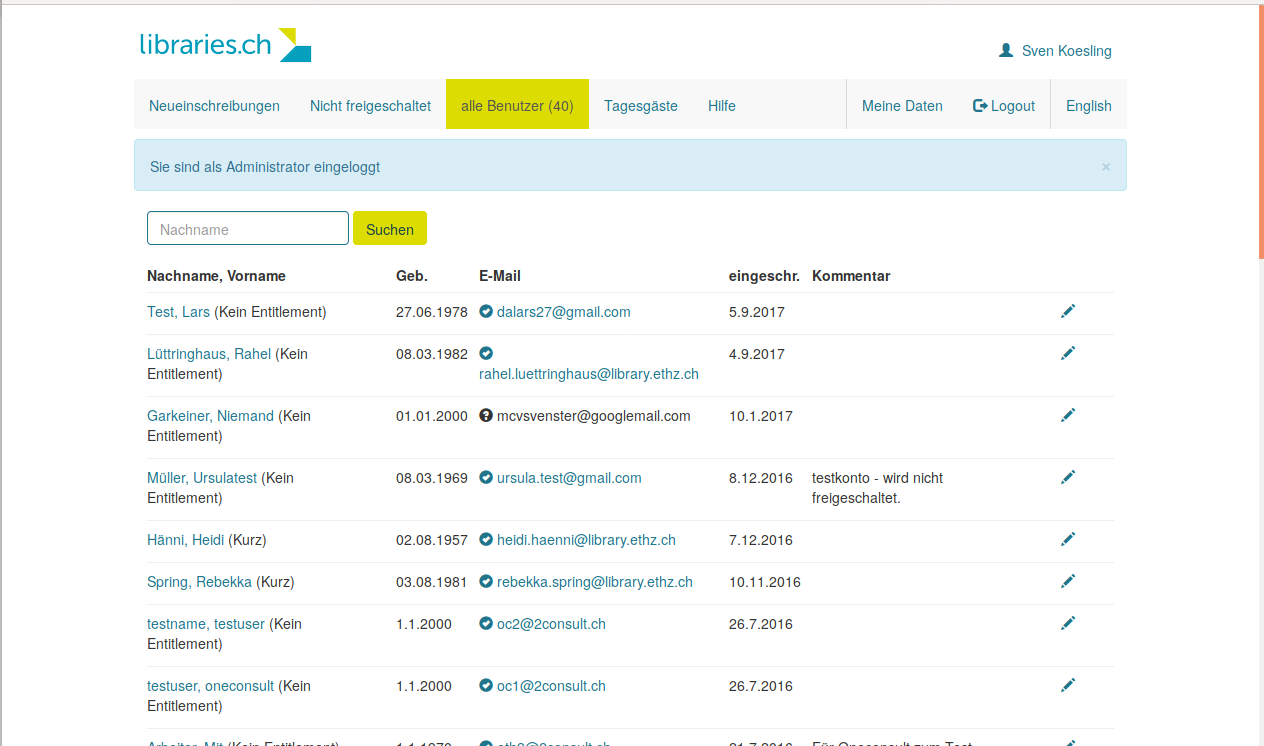
\includegraphics[width=1\textwidth]{pics/bootstrap-normal}
  \end{center}
\end{frame}

\begin{frame}{auf einem mobilen Endgerät}
  \begin{center}
    
\includegraphics[width=0.4\textwidth]{pics/bootstrap-mobile}
  \end{center}
\end{frame}

\only<article>{
  Die vielfältigen UI--Elemente und umfangreichen Funktionen der aktuellen JavaScript--Bibliotheken und --FrameWorks ermöglichen nicht nur komplexe Interaktionen des Benutzers mit der Webseite. In Kombination mit Ajax lassen sich echte Webapplikationen realisieren, die gewöhnlicher Desktop--Software nichts nachsteht. So werden neue Geschäftsmodelle wie Software as a Service erst möglich. 
}

\subsection{Cloud Services}
\label{sub:cloud_services}

\begin{frame}[<+->]{der Einsatz von JavaScript ermöglicht neue Services}
  \begin{itemize}
    \item SaaS
    \item IaaS
    \item PaaS
  \end{itemize}
\end{frame}

\begin{frame}{Beispiel für Saas: iCloud}
  \framesubtitle{Software as a Service}
  \begin{center}
    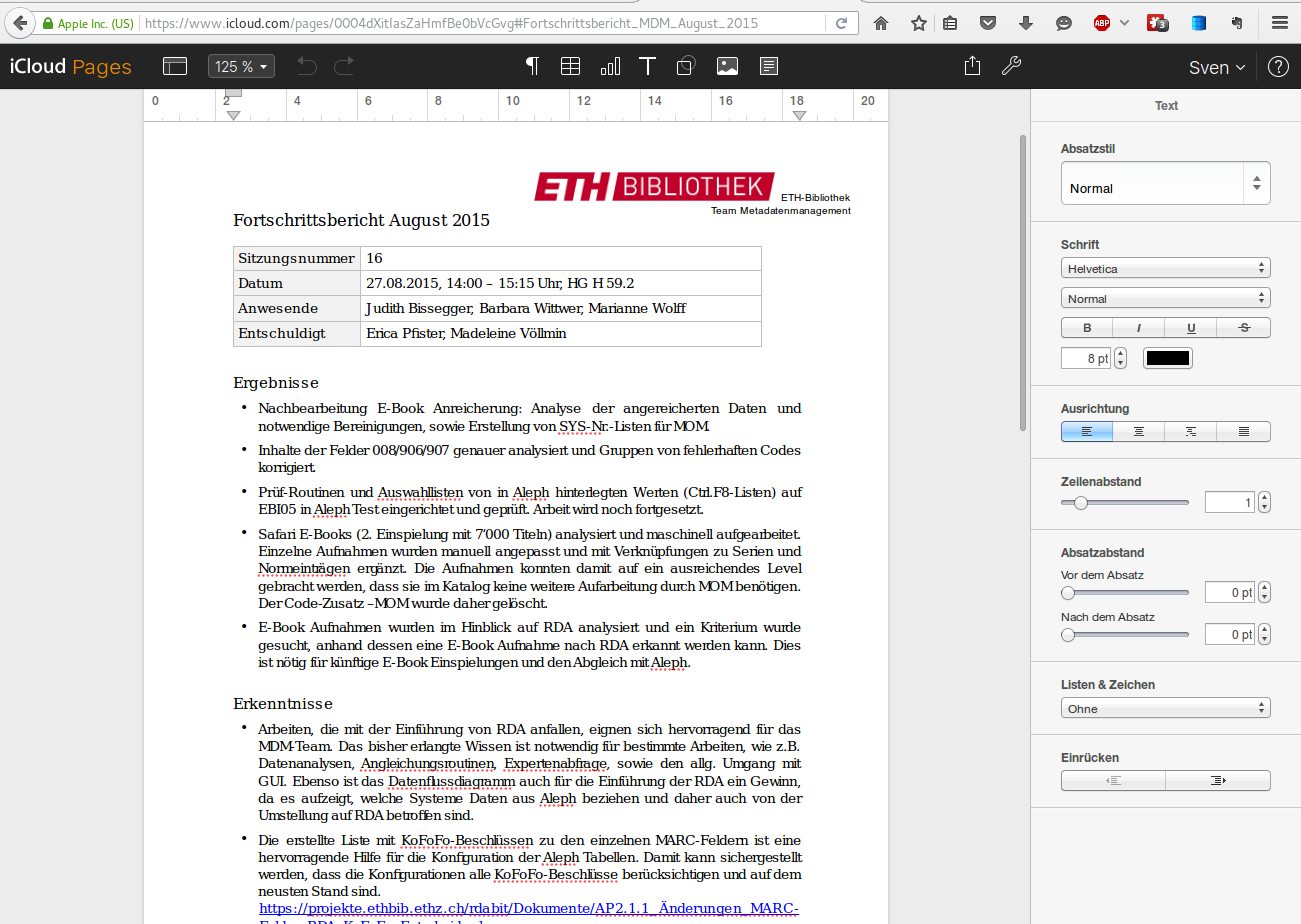
\includegraphics[width=1\textwidth]{pics/SaaS-01-icloud}
  \end{center}
\end{frame}

\begin{frame}{Beispiel für Iaas}
  \framesubtitle{Infrastructure as a Service}
  \begin{center}
    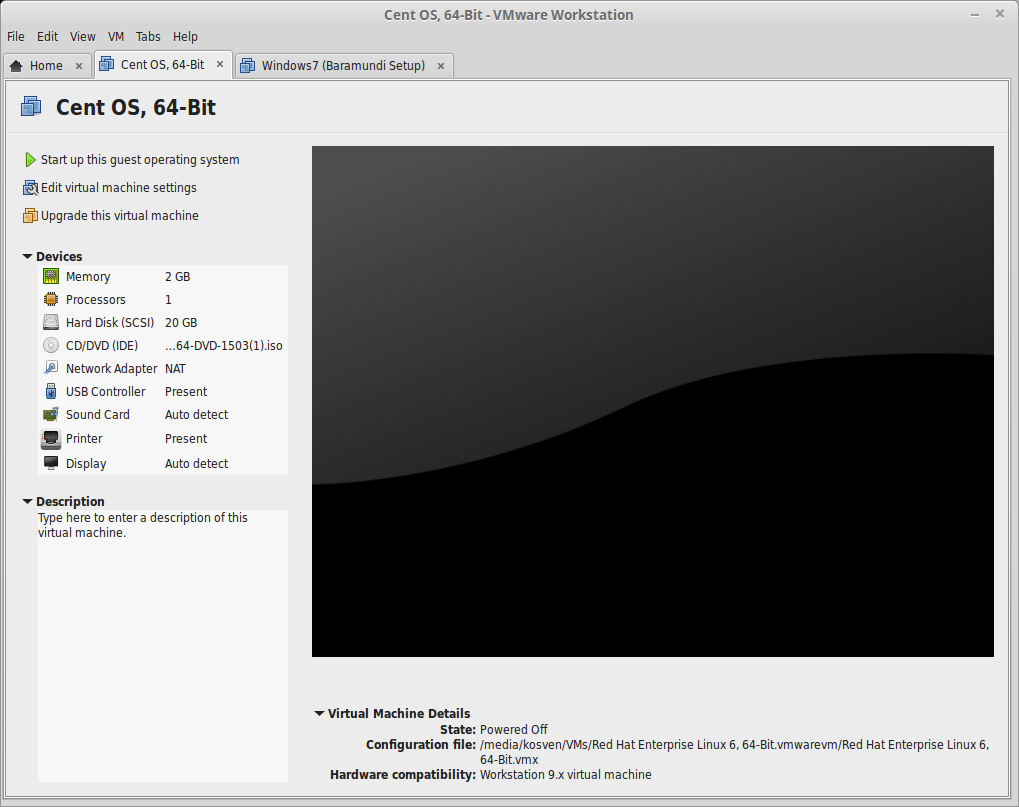
\includegraphics[width=1\textwidth]{pics/IaaS}
  \end{center}
\end{frame}

\begin{frame}{Beispiel für Paas}
  \framesubtitle{Platform as a Service}
  \begin{center}
    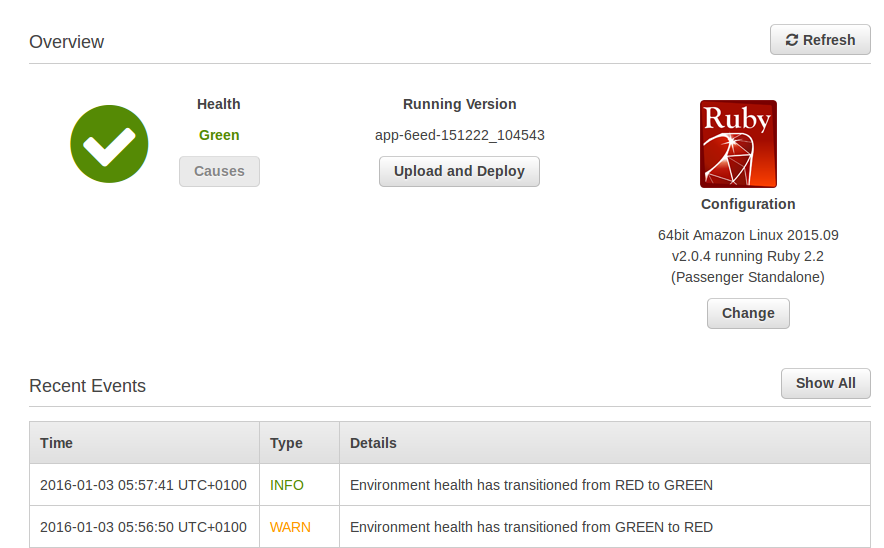
\includegraphics[width=1\textwidth]{pics/PaaS}
  \end{center}
\end{frame}

\subsection{Das DOM für automatisiertes Testen von WebApplikationen verwenden}
\only<article>{
  Nachdem wir das DOM verwendet haben, um vielfältige Funktionen auf einer Webseite zu realisieren, können wir es auch benutzen, um diese Funktionen automatisch vom Computer testen zu lassen.

  Beispielsweise kann man Elemente einer Webseite mit Skriptsprachen auf den korrekten Inhalt prüfen.

  Mittels Ruby und den FrameWorks ,,Cucumber'' und ,,Capybara'' testen wir nach jedem Update von Primo, ob die Features noch so funktionieren, wir wir es geplant haben:
}

\begin{frame}[<+->]{automatisierte Tests von Primo}
  \begin{itemize}
    \item Wir prüfen nach einem Update, ob sich die Suchalgorithmen verändert haben, indem wir die Trefferzahl zwischen den beiden Systemen mit identischem Datenstand vergleichen.
    \item Der Date--Slider hat in der Vergangenheit Probleme gemacht. Wir checken, ob er plausible Ranges liefert.
    \item Wir testen, ob nicht--lateinische Schriftzeichen gefunden werden.
  \end{itemize}
\end{frame}

\only<article>{
  Das Gute an dem verwendeten FameWork ist, dass die Anforderungen nahezu natürlichsprachig formuliert werden. So stellen wir sicher, dass IT und ,,normale'' Menschen vom Gleichen sprechen.
}

\begin{frame}[fragile]{Anforderung in Gherkin formuliert}
  \fontencoding{T1}\selectfont
  \begin{lstlisting}
Szenario: Eine Suche ergibt auf den beiden Prod Systemen eine ähnliche Anzahl Treffer
    Wenn ich die Seite "http://terza-prod1-fe41.ethz.ch/primo-explore/search?vid=DADS&sortby=rank&lang=de_DE" aufrufe,
    Und ich in den Suchschlitz "Wald" eingebe,
    Und die Anzahl der Treffer nehme
    Und dann die Seite "http://terza-prod2-fe41.ethz.ch/primo-explore/search?vid=DADS&sortby=rank&lang=de_DE" aufrufe,
    Wenn ich in den Suchschlitz den Suchbegriff "Wald" eingebe,
    Und dort die Anzahl der Treffer nehme
    Dann sollten die Treffermengen ähnlich, d.h. die Abweichung unter 1%, sein.
  \end{lstlisting}
\end{frame}

\only<article>{
  Schauen wir uns dazu eine Seite im UI von Primo an. Wir wollen in den Suchschlitz das Wort ,,Wald'' eingeben. 
}

\begin{frame}{Der Suchschlitz im alten UI}
  \begin{center}
    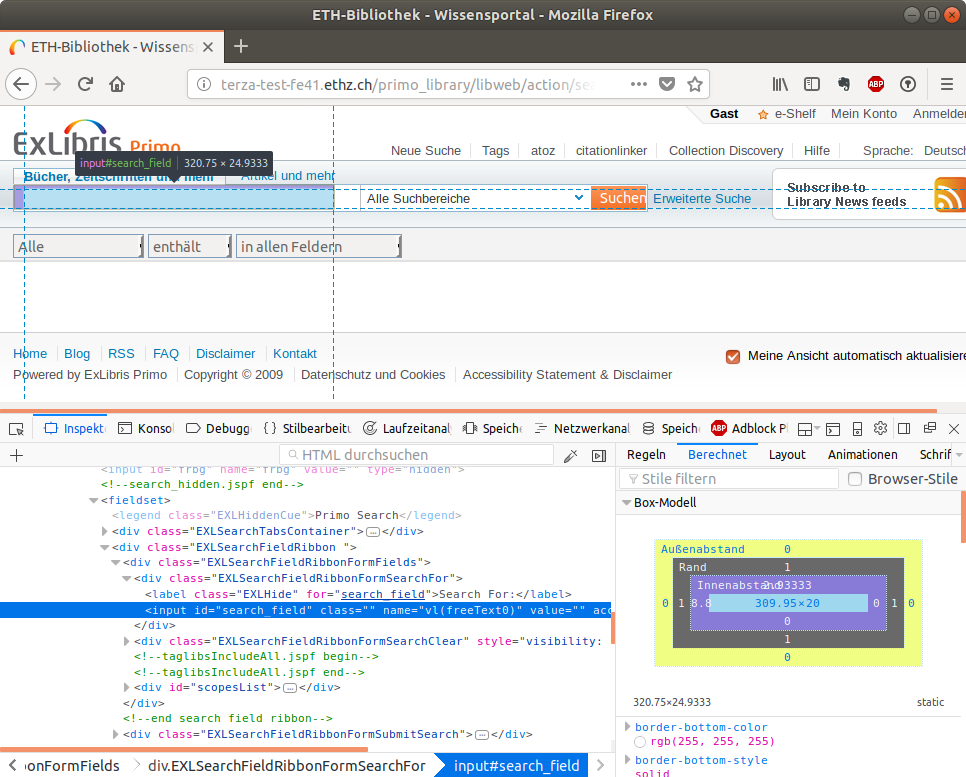
\includegraphics[width=1\textwidth]{pics/old-ui-searchbar}
  \end{center}
\end{frame}

\begin{frame}[fragile]{Quellcode des Suchschlitzes (altes UI)}
  \fontencoding{T1}\selectfont
  \begin{lstlisting}[language=html]
<input name="vl(freeText0)" class="" value="" id="search_field" accesskey="s" type="text">
  \end{lstlisting}
\end{frame}

\only<article>{
  Den Suchschlitz können wir also ansteuern, indem wir im DOM nach der id ,,search_field'' suchen.

  Ein Problem ist, dass sich ids nach Updates ändern können.
}

\begin{frame}{Der Suchschlitz im neuen UI}
  \begin{center}
    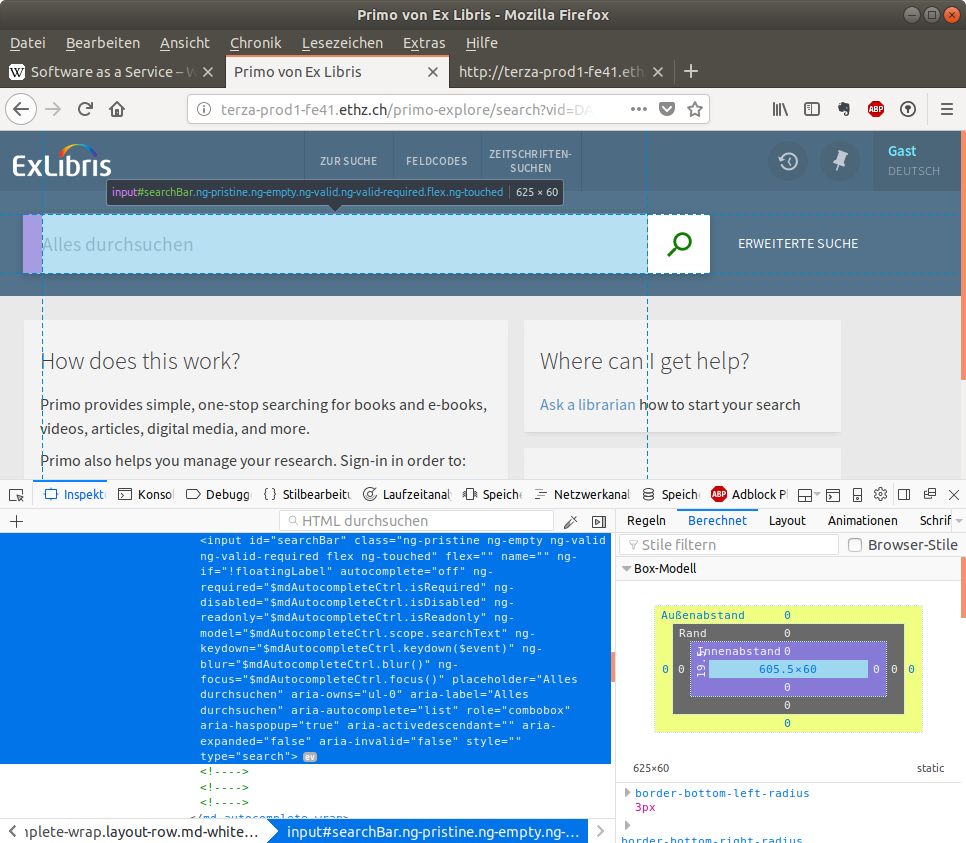
\includegraphics[width=1\textwidth]{pics/pnui-searchbar}
  \end{center}
\end{frame}

\begin{frame}[fragile]{Quellcode des Suchschlitzes (neues UI)}
  \fontencoding{T1}\selectfont
  \begin{lstlisting}[language=html]
<input flex="" id="searchBar" name="" ng-if="!floatingLabel" autocomplete="off" ng-required="$mdAutocompleteCtrl.isRequired" ng-disabled="$mdAutocompleteCtrl.isDisabled" ng-readonly="$mdAutocompleteCtrl.isReadonly" ng-model="$mdAutocompleteCtrl.scope.searchText" ng-keydown="$mdAutocompleteCtrl.keydown($event)" ng-blur="$mdAutocompleteCtrl.blur()" ng-focus="$mdAutocompleteCtrl.focus()" placeholder="Alles durchsuchen" aria-owns="ul-0" aria-label="Alles durchsuchen" aria-autocomplete="list" role="combobox" aria-haspopup="true" aria-activedescendant="" aria-expanded="false" class="ng-pristine ng-empty ng-valid ng-valid-required flex ng-touched" aria-invalid="false" style="" type="search">
  \end{lstlisting}
\end{frame}

\begin{frame}[fragile]{Skript, um ,,Wald'' in den Suchschlitz zu schreiben}
  \fontencoding{T1}\selectfont
  \begin{lstlisting}[language=ruby]
Wenn(/^ich in den Suchschlitz "([^"]*)" eingebe,$/) do |q|
  fill_in('#searchBar', with: q)
  find(".button-confirm").send_keys(:enter)
end
  \end{lstlisting}
\end{frame}


\begin{frame}{Und der Testablauf}
  \begin{center}
    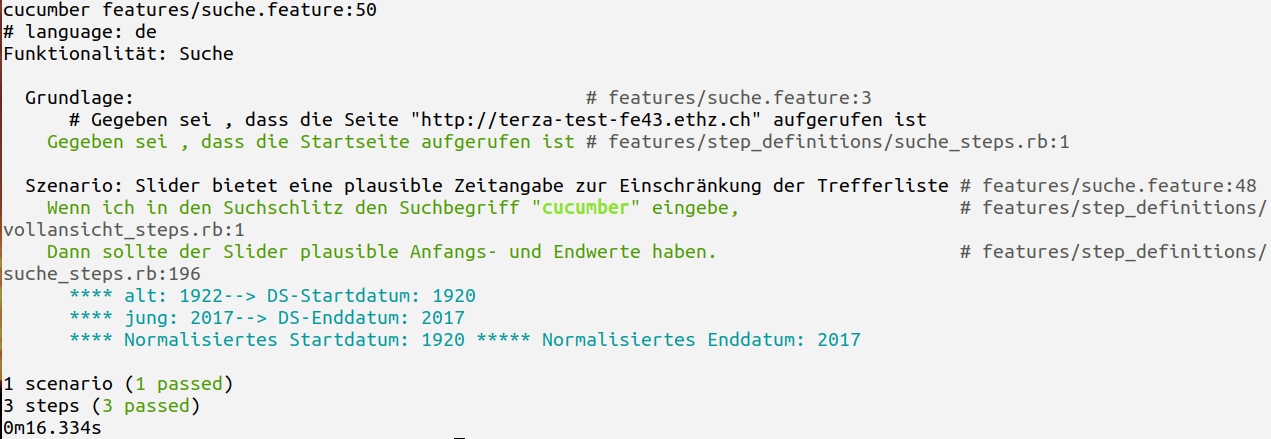
\includegraphics[width=1\textwidth]{pics/cucumber-test}
  \end{center}
\end{frame}
